\documentclass{article}
\usepackage[utf8]{inputenc}
\usepackage[russian]{babel}
\usepackage{hyperref}
\usepackage{underscore}
\usepackage{setspace}
\usepackage{indentfirst} 
\usepackage{mathtools}
\usepackage{amsfonts}
\usepackage{enumitem}
\usepackage{amsthm}
\usepackage[left=2cm,right=2cm,
    top=2cm,bottom=2cm,bindingoffset=0cm]{geometry}
\singlespacing

\usepackage{graphicx}
\graphicspath{ {./images/matan/} }

\newcommand{\bydef}{\stackrel{\text{по опр.}}{\implies}} % by definition - по определению
\newcommand{\parspace}{\vspace{10pt}}

\newcommand{\imagin}{\mathrm{Im} \,}
\newcommand{\real}{\mathrm{Re} \,}

\newcommand{\dslim}{\displaystyle\lim}
\newcommand{\dslimn}{\dslim_{n \to \infty}}

\newcommand{\prop}[1]{#1^{\text{o}}}

\newtheorem{theorem}{Теорема}[section]

\begin{document}

\section{Теория действительного (вещественного) числа}
\subsection{Определение действительного числа}
Назовём вещественным (действительным) числом последовательность
$a_0,a_1 a_2 \dots a_n$ целых чисел, таких, что $0 \le a_i \le 9$,
причём перед ней поставим знак плюс или знак минус,
$a_0$ -- целое неотрицательное число, которое отделяется запятой.
Если перед числом стоит знак плюс, то его называют положительным,
а если знак минус, то отрицательным.

\textbf{Определение}

Рассмотрим действительное число $x = a_0,a_1 a_2 \dots a_m \dots > 0$.
Рациональное число $x = a_0,a_1 a_2 \dots a_m$ называют
\textbf{нижним $m$-значным приближением числа $x$}.
Рациональное число $\overline{x_m} = x_m + \frac{1}{10^m}$ называют
\textbf{верхним $m$-значным приближением числа $x$}.

\[y = -x (x > 0)\]
\[y = -a_0,a_1 a_2 \dots a_m \dots\]
\[y_m = -\overline{x_m}\]
\[\overline{y_m} = -x_m\]

\textbf{Очевидными являются свойства:}
\begin{enumerate}
    \item $x_{m+1} \ge x_m$
    \item $\overline{x_{m+1}} \le \overline{x_m}$
    \item $\forall m,n \quad x_m \le \overline{x_n}$
    \item $x_{m+1} - x_m < \frac{1}{10^m}$
    \item Если существуют такие числа $a$ и $b$, что $b \ge a$
    и разность $b - a < \frac{1}{10^m}$ $\implies$ существует
    вещественное число $x$, что $x_m = a$, нижнее приближение есть число $a$.
\end{enumerate}

\parspace

\textbf{Теорема}. \textit{Соответствие между вещественными числами и точкам прямой}.

Множество вещественных чисел эквивалентно множеству точек прямой в том смысле, что
между этими множествами существуют взаимно однозначные соответствия.

\textbf{Доказательство}.

\begin{enumerate}
    \item (точке $\rightarrow$ число) Точке можно сопоставить число.

    На прямой поставим произвольно две точки $O$ и $E$, где $E$ правее $O$.
    Сопоставим точке $O$ число $0,0 \dots 0 \dots$, а точке $E$
    Сопоставим число $1,0 \dots 0 \dots$.
    
    Пусть точка $M$ правее $O$. Сопоставим ей действительное число
    $x = a_0,a_1 a_2 \dots a_m \dots$ по следующему правилу:
    
    $a_0 = $ максимальному числу отрезков $OE$, укладывающихся внутри $OM$.
    Если при этом остатка нет, то $a_1 = a_2 = \dots = a_m = \dots = 0$.
    
    Если есть остаток $M_1M$, то $a_1$ определим как наибольшее число
    $OE_1 = \frac{1}{10}OE$, укладывающихся внутри отрезка $M_1M$.
    
    Если остатка нет, то $a_2 = \dots = a_m = \dots = 0$, а если остаток есть,
    то продолжаем этот процесс, откладывая отрезки $OE_2 = \frac{1}{100}OE$ 
    и т.д. Таким образом любой точке правее $O$ можно сопоставить действительное
    число $x$, определяя подобным образом любую цифру этого числа.
    
    Если $M$ левее $O$, то поступаем аналогично, но перед числом ставим знак минус.

    \item (числу $\rightarrow$ точка) Каждому числу на прямой можно сопоставить точку.

    Пусть задано некое число $x = a_0,a_1 a_2 \dots a_m \dots$. Считаем, что
    $x$ -- положительное. Пусть числу $0,0 \dots 0 \dots$ соответствует точка $O$.
    Числу $1,0 \dots 0 \dots$ соответствует точка $E$ (правее $O$).
    
    Отложим от точки $O$ вправо точки $M_m$ и $M_m'$, которые соответствуют
    $x_m$ и $\overline{x_m}$. Получим последовательность вложенных друг в друга
    отрезков $M_0M_0', M_1M_1', \dots$, вложенные в том смысле, что каждая
    $M_{m+1}$ лежит не левее $M_m$, и каждая $\overline{M_{m+1}}$ лежит
    не правее $M_m'$. Воспользуемся \underline{\textit{аксиомой Кантора для прямой}}:
    
    ``Для любой последовательности вложенных друг в друга отрезков существует
    по крайней мере одна точка, принадлежащая каждому из этих отрезков.''
    
    Осталось доказать, что для наших вложенных отрезков существует только одна точка.
    
    Допустим от противного, существуют две точки $M$ и $M'$ $\implies$ отрезок
    $MM'$ содержится в любом отрезке $M_mM_m'$. Но длина отрезка $MM'$ -- это
    $\frac{1}{10^m}$, и тогда можно выбрать такое большое $m$, что $\frac{1}{10^m}$
    станет меньше длины отрезка $MM'$, но это противоречит тому, что $MM'$ содержится в
    $M_mM_m'$ $\implies$ для нашей системы вложенных отрезков такая точка единственная и
    именно её и сопоставим числу $x$.
\end{enumerate}

\textbf{Теорема доказана.}

\subsection{Сравнение вещественных чисел}
\textbf{Определение}

Будем говорить, что вещественное число $x$ $>$ вещественного числа $y$ и обозначать
$x > y$ или $y < x$, если $\exists m_0 \ge 0$, что $x_{m_0} > \overline{y_{m_0}}$

\parspace

\underline{\textbf{Замечание 1}}

Так как $x_0 \le x_1 \le x_2 \le \dots$, 
а $\overline{y_0} \ge \overline{y_1} \ge \overline{y_2} \ge \dots$,
то если $x_{m_0} > \overline{y_{m_0}}$, то неравенство $\overline{x_m} > \overline{y_m}$,
выполняется $\forall m \ge m_0$ и поэтому одновременное выполнение
$x > y$ и $y > x$ невозможно.

Иначе допустим, что $x > y$ и $y > x$, тогда
\[\exists m_1 \quad x_m > \overline{y_m} \quad \forall m \ge m_1 \quad (1)\]
\[\exists m_2 \quad y_m > \overline{x_m} \quad \forall m \ge m_2 \quad (2)\]

Тогда для $\forall m \ge \max (m_1, m_2)$ оба неравенство выполняются одновременно.

$x_m \stackrel{(1)}{>} \overline{y_m}
\stackrel{\text{опр.}}{\ge} y_m 
\stackrel{(2)}{>} \overline{x_m} \implies x_m > \overline{x_m}$.
\textbf{Получили противоречие}.

\parspace

\textbf{Определение}

Если для $x, y \in \mathbb{R}$ не выполняется ни одно из неравенств $x > y$ и $y > x$,
то числа называют равными и обозначают $x = y$.

\parspace

\underline{\textbf{Замечание 2}}
Если $x = y$, то для их десятичных приближений возможно лишь одно из соотношений:
$x_m = y_m$, или $\overline{x_m} = y_m$, или $x_m = \overline{y_m}$.

При этом два последних случая возможны если $x = a_0,a_1 \dots a_{l-1}a_l0$,
$y = a_0,a_1 \dots a_{l-1}(a_l-1)9 \dots$ 

Например, если $x = 0.5$, $y = 0.499 \dots$ $\implies x = y$,
поэтому договоримся для чисел
\[a_0,a_1 \dots a_{l-1}a_l0 \quad (1)\]
\[a_0,a_1 \dots a_{l-1}(a_l-1)9 \dots \quad (2)\]

использовать форму (1).

\parspace

\textbf{Теорема}. \textit{Свойство транзитивности операции сравнения}.

а) Если $x > y, y > z \implies x > z$

б) Если $x = y, y = z \implies x = z$

\textbf{Доказательство}.

а) По условию 
\[x > y \implies \exists m_1: x_m > \overline{y_m} \quad \forall m \ge m_1\]
\[y > z \implies \exists m_2: y_m > \overline{z_m} \quad \forall m \ge m_2\]
$\implies \forall m \ge \max (m_1, m_2)$ выполняется $x_m > \overline{y_m}$
и $y_m > \overline{z_m}$, т.е. $x_m > \overline{y_m} > y_m > \overline{z_m}$,
т.е. $x_m > \overline{z_m} \implies x > z$.

б) По условию 
\[x = y \implies \exists m_1: x_m = y_m \quad \forall m \ge m_1\]
\[y = z \implies \exists m_2: y_m = z_m \quad \forall m \ge m_2\]
$\implies \forall m \ge \max (m_1, m_2)$ выполняется $x_m = y_m$
и $y_m = z_m$, т.е. $x_m = y_m = z_m$,
т.е. $x_m = z_m \implies x = z$.

\pagebreak

\subsection{Признак равенства действительных чисел}

\textbf{Теорема}.

Если для данных чисел $x$ и $y$ и 
$\forall \varepsilon > 0 \quad \exists \alpha_{\varepsilon}, \beta_{\varepsilon}$
с конечным числом десятичных знаков, такие, что
$\alpha_{\varepsilon} \le x \le \beta_{\varepsilon}, \alpha_{\varepsilon} \le y \le \beta_{\varepsilon}$
и $\beta_{\varepsilon} - \alpha_{\varepsilon} < \varepsilon$, тогда $x = y$.

\textbf{Доказательство}.

Допустим от противного, условие теоремы выполняется, но 
$y > x \bydef \exists m_0: y_{m_0} > \overline{x_{m_0}}$

Имеем $\alpha_{\varepsilon} \le x \le \overline{x_{m_0}} < y_{m_0} \le y \le \beta_{\varepsilon}$
и это справедливо $\forall m \ge 0$, т.е. 
$\alpha_{\varepsilon} \le \overline{x_m} < y_m \le \beta_{\varepsilon}$
$\implies 0 < y_m - \overline{x_m} \le \beta_\varepsilon - \alpha_\varepsilon < \varepsilon$,
но $y_m - \overline{x_m}$ не может быть меньше, чем $\frac{1}{10^m}$. А если взять
$\varepsilon < \frac{1}{10^m} (\varepsilon > 0)$, то \textbf{получим противоречие}
$\implies y_m = \overline{x_m}$.

Аналогично рассуждая для $x > y \implies x_m = \overline{y_m}$, значит невозможно
ни $x > y$, ни $y > x$ $\bydef x = y$.

\section{Численные множества}

\subsection{Точные грани численного множества}

\begin{itemize}
    \item $[a;b]$ -- отрезок $= \{x | a \le x \le b\}$
    \item $(a;b)$ -- интервал $= \{x | a < x < b\}$
    \item $(a;b]$ -- полуинтервал $= \{x | a < x \le b\}$
    \item $[a;b)$ -- полуинтервал $= \{x | a \le x < b\}$
\end{itemize}

$\mathbb{N} \subset \mathbb{Z} \subset \mathbb{Q} \subset \mathbb{R}$

\subsection{Ограниченность}

Числовое множество $A$ называют ограниченным сверху, если 
$\exists M \in \mathbb{R}: \forall x \in A$ выполняется $x \le M$,
число $M$ называется \textbf{мажорантой} множества $A$.

Числовое множество $A$ называют ограниченным снизу, если 
$\exists m \in \mathbb{R}: \forall x \in A$ выполняется $x \ge m$,
число $m$ называется \textbf{минорантой} множества $A$.

Множество $A$ называется ограниченным, если оно ограничено сверху или снизу,
т.е. $\exists m, M \in \mathbb{R}: \forall x \in A$ выполняется $m \le x \le M$
(или $\exists C > 0: \forall x \in A$ выполняется $|x| \le C$).

\parspace

\textbf{Определение}.

Наименьшая мажоранта множества $A$ называется верхней гранью $A$ и обозначается
$\sup A$ (супремум).

Наибольшая миноранта множества $A$ называется нижней гранью $A$ и обозначается
$\inf A$ (инфимум).

% \subsection{Метод математической индукции}

% Говорят, что утверждения $A_{n_0}, A_{n_0 + 1}, \dots, A_{n_0 + n}, \dots$ являются
% истинными по методу математической индукции (ММИ), если выполняются два утверждения:
% \begin{enumerate}
%     \item $A_{n_0}$ -- истина (база индукции)
%     \item Если $A_k$ -- истина, то $A_{k+1}$ -- истина (шаг индукции)
% \end{enumerate}

\subsection{Признак верхней и нижней грани множества}.

$M = \sup A$, если 
\begin{enumerate}
    \item $\forall x \in A \quad x \le M$
    \item $\forall M' < M \quad \exists x_0 \in A: x_0 > M'$
    (или $\forall \varepsilon > 0 \quad \exists x_\varepsilon \in A: x_\varepsilon > M - \varepsilon$)
\end{enumerate}

$m = \inf A$, если 
\begin{enumerate}
    \item $\forall x \in A \quad x \ge m$
    \item $\forall m' > m \quad \exists x_0 \in A: x < m'$
    (или $\forall \varepsilon > 0 \quad \exists x_\varepsilon \in A: x_\varepsilon < m + \varepsilon$)
\end{enumerate}

\textbf{Теорема}. \textit{О существовании верхней грани (нижней грани)}.

У всякого непустого ограниченного сверху множества существует верхняя грань (нижняя грань).

\textbf{Доказательство}.

Множество $A$ -- ограничено сверху $\implies \exists b \in \mathbb{R}: \forall x \in A:
x \le b, A \ne 0 \implies \exists a \in A$ и $a \le b$.

Рассмотрим такие элементы $x \in A: a \le x \le b$. Рассмотрим их $x_m$ приближения.
Число таких $x$ может быть бесконечным, но число $x_m$ -- конечно.
(их не более, чем $(b_m - a_m) * 10^m$). 

Тогда обозначим $C_m = \max (x_m) (x \in A; a \le x \le b)$.
Так как $x_{m+1} - x_m < \frac{1}{10^m} \implies C_{m+1} - C_m < \frac{1}{10^m}$
$\stackrel{\text{по св-ву}}{\implies} C_m$ -- нижние $m$-значные приближения некоторого 
действительного числа $C$.

Докажем, что $C = \sup A$ по признаку.
\begin{enumerate}
    \item Надо доказать $\forall x \in A: x \le C$
    
    Допустим от противного: $\exists x_0 \in A: x_0 > C \stackrel{\text{по опр}}{\implies}
    \exists m_1: \forall m \ge m_1 \quad (x_0)_m > \overline{C_m}$, но
    $\overline{C_m} \ge C_m \implies (x_0)_m > C_m$, а это противоречит выбору $C_m$
    $\implies \forall x \in A: x \le C$.

    \item Возьмём $\forall C' < C \bydef C_m > \overline{C_m'} \ge C'$.
    Но по выбору $C_m = (x_0)_m \quad (x_0 \in A, a \le x_0 \le b)$.
    Имеем: $x_0 \ge (x_0)_m = C_m > \overline{C_m'} \ge C' \implies x_0 > C'$,
    т.е. $\forall C' < C \quad \exists x_0 \in A: x_0 > C'$.
    $\implies$ по признаку верхней грани $C = \sup A$.
\end{enumerate}

\textbf{Теорема доказана}.

\parspace

\underline{\textbf{Замечание 1.}}

В ходе доказательства были получены неравенства: $\forall x \in A$
\[x_m \le (\sup A)_m \le \sup A\]
\[\overline{x_m} \ge \overline{(\inf A)_m} \ge \inf A\]

\parspace

\underline{\textbf{Замечание 2.}}

Если множество $A$ не ограничено сверху, то $\sup A = + \infty$, а если множество $A$
не ограничено снизу, то $\inf A = - \infty$.

\parspace

\textbf{Теорема}. \textit{Свойство граней}.

Если $\forall x \in A \quad \forall y \in B: x \le y \implies \sup A \le \inf B$

\textbf{Доказательство}.

По условию $\forall y \in B \quad y \ge x \implies x$ -- миноранта $B$
$\implies \inf B \ge x$, т.е. $\forall x \in A \quad x \le \inf B \implies \inf B$ --
мажоранта $A$ $\implies \sup A \le \inf B$. \textbf{Теорема доказана}.

\section{Арифметические операции для действительных чисел}

\textbf{Определение}.

Рассмотрим множество \underline{всех} таких чисел
$\alpha_1, \alpha_2, \beta_1, \beta_2$ с конечным числом десятичных знаков
после запятой, что
\[\alpha_1 \le x \le \alpha_2\]
\[\beta_1 \le y \le \beta_2\]

Тогда суммой чисел $x$ и $y$ ($x, y \in \mathbb{R}$) назовём число 
$(x + y) = \sup (\alpha_1 + \beta_1) = \inf (\alpha_2 + \beta_2)$

Пусть теперь $x \ge 0, y \ge 0$, тогда произведением неотрицательное $x$ и $y$
назовём число $(x * y) = \sup (\alpha_1 * \beta_1) = \inf (\alpha_2 * \beta_2)$.
Действия с отрицательными числами определим так же, как и для рациональных чисел.

Разностью $x$ и $y$ ($x, y \in \mathbb{R}$) назовём число $(x - y) = x + (-y)$.

Частным чисел $x$ и $y$ ($x \in \mathbb{R}, y > 0$) назовём число 
$\frac{x}{y} = x * \frac{1}{y}$, где $\frac{1}{y} = \inf \frac{1}{\beta_1}$.
Для $y < 0$ -- $\frac{x}{y} = -x * \frac{1}{-y}$.

\parspace

\underline{\textbf{Свойства арифметических операций}}
\begin{enumerate}
    \item $a + b = b + a$ (коммутативность сложения)
    \item $a * b = b * a$ (коммутативность умножения)
    \item $(a + b) + c = a + (b + c)$ (ассоциативность сложения)
    \item $(a * b) * c = a * (b * c)$ (ассоциативность умножения)
    \item $\forall a \in \mathbb{R} \quad a + 0 = a$ 
    (существование нейтрального элемента сложения)
    \item $\forall a \in \mathbb{R} \quad a * 1 = a$
    (существование нейтрального элемента умножения)
    \item $a + (-a) = 0$
    \item $a * \frac{1}{a} = 1$ ($a \neq 0$)
    \item $(a + b) * c = a * c + b * c$ (дистрибутивность)
    \item Если $a < b \implies a + c < b + c$
    \item Если $a < b, c > 0 \implies a * c < b * c$,
    
    Если $a < b, c < 0 \implies a * c > b * c$
    \item \textbf{Аксиома Архимеда}
    
    \textit{Каково бы ни было действительное число $a$, единицу можно столько
    раз повторить слагаемым, что полученная сумма превзойдет число $a$}
\end{enumerate}

\section{Степени действительных чисел}

Пусть $a \in \mathbb{R}, a > 0$

\begin{enumerate}
    \item $x \in \mathbb{N}, x = n \\
    a^x = a^n = \underbrace{a * \dots * a}_n$
    \item $x \in \mathbb{Z}$
    
    $
    \begin{cases}
        x = n & \implies \text{см. 1} \\
        x = -n & \implies a^{-n} = \frac{1}{a^n} \\
        x = 0 & \implies a^0 = 1
    \end{cases}
    $

    \item $x \in \mathbb{Q}, x = \frac{m}{n} \quad m \in \mathbb{Z}, n \in \mathbb{N}\\
    a^{\frac{1}{n}} = \sqrt[n]{a} = b \Leftrightarrow b^n = a\\
    a^{\frac{m}{n}} = \sqrt[n]{a^m}$
    \item Пусть $x \in \mathbb{R}^+$ и $x_m, \overline{x_m}$ -- его $m$-значное приближение.
    
    $ a^x =
    \begin{cases}
        \sup a^{x_m}, & \text{если } a > 1 \\
        \frac{1}{(\frac{1}{a})^x}, & \text{если } 0 < a < 1
    \end{cases}
    $
\end{enumerate}

Во всех определениях $a^x$ обладает \textbf{свойствами}:
\begin{enumerate}
    \item $x_1 < x_2
    \begin{cases}
        a^{x_1} > a^{x_2}, & \text{если } 0 < a < 1 \\
        a^{x_1} < a^{x_2}, & \text{если } a > 1
    \end{cases}
    $

    \item $a^{x_1}*a^{x_2} = a^{x_1 + x_2} \\
    \frac{a^{x_1}}{a^{x_2}} = a^{x_1 - x_2}$
    \item $(a^{x_1})^{x_2} = a^{x_1 * x_2}$
    \item $a^x * b^x = (a * b)^x \\
    \frac{a^x}{b^x} = (\frac{a}{b})^x$
\end{enumerate}

\section{Предельные точки числового множества}

\textbf{Определение}

Множество $x \in \mathbb{R}$, удовлетворяющих неравенству $|x - a| < \varepsilon$
называется $\varepsilon$-окрестностью точки $a$.

$|x| < c \Leftrightarrow -c < x < c$

$|x - a| < \varepsilon \Leftrightarrow -\varepsilon < x - a < \varepsilon \Leftrightarrow
a - \varepsilon < x < a + \varepsilon \Leftrightarrow x \in (a - \varepsilon, a + \varepsilon)$.

\parspace

\textbf{Определение}

Точка $x$ называется \textbf{предельной} точкой множества $A$, если в любой $\varepsilon$-окрестности
точки $x$ находится точки множества $A$, отличные от $x$.

\parspace

\underline{\textbf{Замечание}}

Можно показать, что если точка $x$ -- предельная точка множества $A$, то в любой её
$\varepsilon$-окрестности находится бесконечное число элементов $A$.

Допустим, что это не так и у точки $x$ в некоторой окрестности содержится конечное
число элементов множества $A$ ($x_1,x_2,\dots,x_n \in A$).

Выберем такой элемент, что $|x - x_j|$ был $\underset{1 \le k \le n}{\min} |x - x_k|$,
тогда в $\varepsilon_1$-окрестности, где $\varepsilon_1 = \frac{|x - x_j|}{2}$ нет ни
одного элемента множества, отличного от $x$ $\implies$ $x$ не предельная точка множества
$A$, а это противоречит условию.

\parspace

\textbf{Определение}

Точка $x \in A$ называется \textbf{изолированной} точкой множества $A$, если найдется такая
окрестность точки $x$, в которой не найдется ни одного элемента множества $A$,
кроме неё самой.

\parspace

\textbf{Определение}

Точка $x$ называется \textbf{внутренней} точкой множества $A$, если найдется такая
окрестность точки $x$, которая целиком содержится во множестве $A$.

\parspace

\textbf{Определение}

Множество, все точки которого внутренние называется \textbf{открытым} множеством.

\parspace

\textbf{Определение}

Множество, которое содержит все свои предельные точки называется замкнуным множеством.

\parspace

\textbf{Теорема}. \textit{О существовании предельных точек (Теорема Больцано-Вейерштрасса для множеств)}.

У всякого бесконечного ограниченного числового множества существует по крайней мере
одна предельная точка.

\textbf{Доказательство}.

Докажем, что существует самая правая предельная точка.

$A$ -- ограниченное $\bydef \exists C > 0 \quad
\forall x \in A: |x| \le C$
$C$ без ограничения общности можно выбрать целым.
Рассмотрим отрезок вида $[k;k+1]$, удовлетворяющий $-c \le k \le c - 1$.
Так как $A$ -- бесконечное, то по крайней мере в одном из этих отрезков содержится
бесконечное количество элементов множества $A$.

Выберем самый правый из них и обозначим его $[y_0;\overline{y_0}]$.
Разобьём его на 10 равных частей $\implies$ по крайней мере в одном из
полученных отрезков содержится бесконечное число элементов множества $A$.

Выберем самый правый из них и обозначим его $[y_1;\overline{y_1}]$.
Продолжим процесс деления отрезок на 10 частей и выберем самый правый отрезок
на котором содержится бесконечное число элементов множества $A$.

Получим отрезок $[y_m;\overline{y_m}]$, где $m = 0,1,\dots$, причём неравенству
$x > \overline{y_m}$ может удовлетворять только конечное число элементов $A$,
длина каждого отрезка $= \frac{1}{10^m}$ и концы отрезков удовлетворяют
следующим неравенствам:

\[y_{m+1} \ge y_m\]
\[\overline{y_{m+1}} \le \overline{y_m}\]
\[y_{m+1} - y_m < \frac{1}{10^m}\]
\[\overline{y_m} - y_m = \frac{1}{10^m}\]

Тогда они являются нижним и верхним $m$-значным приближением некоторого числа $y$.

Покажем, что оно является предельной точкой $A$. Возьмём любую $\varepsilon$-окружность
точки $y$ и выберем такое $m$, чтобы: 
$\frac{1}{10^m} < \varepsilon \implies [y_m;\overline{y_m}] \subset 
(y - \varepsilon; y + \varepsilon)$, но он содержит бесконечное число элементов
множества $A$ $\bydef$ $y$ являлся предельной точкой
множества $A$, а так как правее $\overline{y_m}$ находится только конечное число
элементов $A$, то $y$ -- самая правая предельная точка $A$.

\textbf{Теорема доказана.}

\section{Множество комплексных чисел}

\subsection{Определение комплексного числа}

\textbf{Комплексным числом} $z$ будем называть упорядоченную пару действительных
чисел $(x;y)$ такую, что для этих пар определены понятия равенства и арифметических
операций следующим образом:

\begin{enumerate}
    \item Если $\\ z_1 = (x_1;y_1) \\ z_2 = (x_2;y_2)$, то
    
    $z_1 = z_2 \Leftrightarrow \begin{cases}
        x_1 = x_2 \\
        y_1 = y_2
    \end{cases}$

    \item $z_3 = z_1 + z_2 \Leftrightarrow z_3 = (x_1 + x_2; y_1 + y_2)$
    \item $z_3 = z_1 - z_2 \Leftrightarrow z_3 = (x_1 - x_2; y_1 - y_2)$
    \item $z_3 = z_1 * z_2 \Leftrightarrow z_3 = (x_1 x_2 - y_1 y_2; x_1 y_2 + x_2 y_1)$
    \item $z_3 = \frac{z_1}{z_2} (z_2 \neq (0; 0)) \Leftrightarrow 
    z_3 = (\frac{x_1 x_2 + y_1 y_2}{x_2^2 + y_2^2}; \frac{x_2 y_1 - x_1 y_2}{x_2^2 + y_2^2})$
\end{enumerate}

Множество комплексных чисел обозначается $\mathbb{C}$.

\parspace

\underline{\textbf{Замечание}}
\begin{enumerate}
    \item Во множестве комплексных чисел операции $>, <$ не имеют смысла.
    \item $z = (x; 0)$ будем называть действительными числами и обозначать $x$.
    \item Заметим:

    $(0; 1) * (0; 1) = (0 - 1; 0 + 0) = (-1; 0) = -1 \\
    (0; 1)^2 = 1 \\ (0; 1)$ -- обозначается $i$ -- мнимая единица.

    $i^2 = -1$

    \item $z = (x; y) = (x; 0) + (0; y) = x + (y; 0) * (0; 1) = x + y * i$

    $z = x + iy$ -- \textbf{алгебраическая форма записи комплексного числа}.

    \item В паре $z = (x; y)$, $x$ называют действительной (вещественной)
    частью и обозначается $x = Re(z)$

    $y$ называют мнимой частью и обозначается $y = Im(z)$

    $z = Re(z) + i*Im(z)$

    \item Комплексное число $Re(z) - i*Im(z) = \overline{z}$ и называется
    сопряжённым к числу $z$, т.е. $z = (x;y), \overline{z} = (x; -y)$.
    \begin{enumerate}[label*=\arabic*.]
        \item $\overline{z_1 \pm z_2} = \overline{z_1} \pm \overline{z_2}$
        \item $\overline{z_1 z_2} = \overline{z_1} * \overline{z_2}$
        \item $\overline{\frac{z_1}{z_2}} = \frac{\overline{z_1}}{\overline{z_2}}$
        \item $\overline{\overline{z}} = z$
        \item $Re(z) = \frac{z + \overline{z}}{2}; Im(z) = \frac{z - \overline{z}}{2i}$
    \end{enumerate}
\end{enumerate}

\subsection{Геометрическое толкование комплексного числа как точки плоскости}

\textbf{ВСТАВИТЬ ГРАФИК???}

\[z = |z|(\cos \phi + i \sin \phi)\]
\[|z| = \sqrt{Re^2(z) + Im^2(z)} = \sqrt{x^2 + y^2}\]

Угол, который радиус-вектор образует с положительной осью $Re(z)$
называют аргументом $z$.

\[\phi = \textnormal{Arg}(z)\]
\[
    \begin{cases}
        \cos \phi = \frac{Re(z)}{|z|} \\
        \sin \phi = \frac{Im(z)}{|z|}
    \end{cases}
\]

При этом $\phi \in (-\pi; \pi]$ называют главным значением аргумента и обозначают $\arg z$
\[Arg(z) = \arg z + 2 \pi k, k \in \mathbb{Z}\]

\parspace

\underline{\textbf{Замечание}}

\begin{enumerate}
    \item Очевидно, $|Re(z)| \le |z|; |Im(z)| \le |z|$
    \item $|z|^2 = x^2 + y^2 = (x + iy)(x - iy) = z * \overline{z}$
    \item Из связи прямоугольной и полярной системы координат 
    
    $\implies Re(z) = |z| \cos (Arg(z)), Im(z) = |z| \sin (Arg(z)) \\
    z = Re(z) + i*Im(z) = |z|(\cos \phi + i \sin \phi)$ -- \textbf{тригонометрическая
    форма записи комплексного числа}.
\end{enumerate}

\subsection{Показательная форма записи комплексного числа}

Рассмотрим функцию Эйлера:

$e^{i \phi} = \cos \phi + i \sin \phi$

\parspace

\textbf{Теорема.} \textit{Свойства функции Эйлера.}

\begin{enumerate}
    \item $e^{i \phi_1} * e^{i \phi_2} = e^{i(\phi_1 + \phi_2)}$
    \item $\frac{e^{i \phi_1}}{e^{i \phi_2}} = e^{i(\phi_1 - \phi_2)}$
    \item $(e^{i \phi})^n = e^{i n \phi} \quad (n \in \mathbb{N})$
\end{enumerate}

\textbf{Доказательство.}

\begin{enumerate}
    \item
    \item
    \item
\end{enumerate}

\textbf{Теорема доказана.}

\parspace

Введя функцию Эйлера:

$z = |z| (\cos \varphi + i \sin \varphi) \quad z = |z| e^{i \varphi}$

\underline{\textbf{Замечание:}}

\begin{align*}
    z_1 &= |z_1| e^{i \varphi_1} \quad \varphi_1 = \textnormal{Arg} z i \\
    z_2 &= |z_2| e^{i \varphi_2} \\
    z_1 * z_2 &= |z_1| |z_2| e^{i (\varphi_1 + \varphi_2)} \\
    \frac{z_1}{z_2} &= \frac{|z_1|}{|z_2|} e^{i (\varphi_1 - \varphi_2)}, \, z_2 \ne 0 \\
    \textnormal{Arg} (z_1 * z_2) &= \textnormal{Arg} z_1 + \textnormal{Arg} z_2 \\
    \textnormal{Arg} (\frac{z_1}{z_2}) &= \textnormal{Arg} z_1 - \textnormal{Arg} z_2 \\
    \textnormal{Хотя } \textnormal{arg} (z_1 * z_2) &= \textnormal{Arg} z_1 + \textnormal{Arg} z_2 \textnormal{ не всегда}
\end{align*}

\underline{\textbf{Свойства $|z|$:}}

\begin{enumerate}
    \item $|z| \ge 0$
    \item $|z_1 * z_2| = |z_1| * |z_2|$
    
    $\left| \frac{z_1}{z_2} \right| = \frac{|z_1|}{|z_2|} \quad (z_2 \ne 0)$

    \item Неравенство $\triangle$
    
    $\left| |z_1| - |z_2| \right| \le |z_1 \pm z_2| \le |z_1| + |z_2|$
    
    $|z_1 \pm z_2|^2 = (z_1 \pm z_2) * \overline{(z_1 \pm z_2)} 
    = (z_1 \pm z_2) (\overline{z_1} \pm \overline{z_2})
    = z_1 * \overline{z_1} + z_2 * \overline{z_2} \pm (z_2 * \overline{z_2} + z_1 * \overline{z_1})
    = |z_1|^2+|z_2|^2 \pm 2 \real (z_2 * \overline{z_1})$

    $\real (z_2 * \overline{z_1}) \le |z_2 * \overline{z_1}| = |z_2| |\overline{z_1}| = |z_1| * |z_2|$

    $(|z_1|-|z_2|)^2 \le |z_1 \pm z_2| \le (|z_1| + |z_2|)^2
    = | |z_1| - |z_2| | \le |z_1 \pm z_2| \le |z_1| + |z_2|$
\end{enumerate}

\section{Сфера Римана}

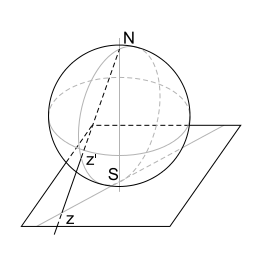
\includegraphics[scale=0.5]{riemannsphere}

Рассмотрим плоскость $XoY$. Точка $O$ -- южный полюс сферы, диаметрально
противоположный точке $P$ -- северному полюсу сферы. Таким образом каждой
точке полскости можно сопоставить каждую точку сферы и, наоборот, каждой 
точке сферы можно сопоставить каждую точку плоскости. Стереографическая проекция
$z$ -- $\infty$ -- бесконечно удаленная точка.

Комплексая плоскость.

\section{Векторы пространства $\mathbb{R}^m$}

\textbf{Определение}

Упорядоченную систему ($x_1, x_2, \dots, x_m$)($x_i \in \mathbb{R}$)
(или ($z_1, z_2, \dots, z_m$); $z_i \in \mathbb{C}$) будем называть вектором
(или точкой) пространства $\mathbb{R}^m (\mathbb{C}^m)$ если для этих
систем определены понятия равенства и арифметические операторы сложения
и умножения на число следующим образом:

Имеем $u(u_1, u_2, \dots, u_m), v(v_1, v_2, \dots, v_m)$:

\begin{enumerate}
    \item $u = v \Leftrightarrow u_i = v_i \quad \forall i = \overline{1, m}$
    \item $u + v = w$, где $w = (u_1 + v_1; u_2 + v_2; \dots; u_m + v_m)$
    \item $k \in \mathbb{R} (k \in \mathbb{C}) \\
    ku = w$, где $w = (k u_1, k u_2, \dots, k u_m)$
\end{enumerate}

Число $u_k$ называется $k$-й компонентой вектора $u$.

\parspace

\textbf{Свойства векторов}

\begin{enumerate}
    \item $u + v = v + u$
    \item $u + (v + w) = (u + v) + w$
    \item $u + v = u + w \Leftrightarrow v = w$
    \item $c * (u + v) = c * u + c * v \quad$ ($c$ -- const)
    \item $u * (c_1 + c_2) = u c_1 + u c_2 \quad$ ($c_1, c_2$ -- const)
    \item $c_1 * (c_2 * u) = (c_1 * c_2) * u \quad$ ($c_1, c_2$ -- const)
\end{enumerate}

\parspace

\textbf{Определение}

Скалярным произведением векторов $u(u_1, u_2, \dots, u_m), v(v_1, v_2, \dots, v_m)$
называют число $u * v = \displaystyle\sum_{k = 1}^{m} u_k * \overline{v_k}$

\parspace

\textbf{Свойства скалярного произведения}
\begin{enumerate}
    \item $u * v = \overline{u * v}$
    \item $(\alpha u + \beta v) * w = \alpha (u * w) + \beta (v * w)$

    ($\alpha, \beta$ -- const)

    $u * (\alpha v + \beta w) = \overline{\alpha} (u * v) + \overline{\beta} (u * w)$

    \item $u * u \ge 0 \quad \forall u$, и $u * u = 0 \Leftrightarrow u = (0,0,\dots,0)$
\end{enumerate}

\parspace

\textbf{Теорема}. \textit{Неравенство Коши-Буняковского}.

$|u v| \le \sqrt{(u * u) * (v * v)}$

\textbf{Доказательство}.

Возьмём $\forall \lambda $ -- const

\begin{enumerate}
    \item $(u + \lambda v) (u + \lambda v) \ge 0$
    \item $(u + \lambda v) u + \overline{\lambda} (u + \lambda v) v \ge 0$
    \item $(u * u) + \lambda (v * u) + \overline{\lambda} (u * v) + \overline{\lambda} * \lambda (v * v) \ge 0$
    \item $(u * u) + \lambda (v * u) + \overline{\lambda} (u * v) + |\lambda|^2 (v * v) \ge 0$
    \item Возьмём $\lambda = \frac{(u * v)}{(v * v)} \quad (v \neq (0, \dots, 0))$
    \item $(u * u) - \frac{(u * v) (v * u)}{(v * v)} - \frac{\overline{(u * v)} (u * v)}{\overline{(v * v)}}
    + \frac{(u * v)^2}{(v * v)^2} (v * v) \ge 0$
    \item $(u * u) - 2 \frac{|(u * v)^2|}{(v * v)} + \frac{(u * v)^2}{(v * v)} \ge 0$
    \item $(u * u) - \frac{|u * v|^2}{(v * v)} \ge 0$
    \item $|u * v| \le \sqrt{(u * u) (v * v)}$
\end{enumerate}

\textbf{Теорема доказана}.

\parspace

\textbf{Определение}.

Модулем вектора $u$ называют число $|u| = \sqrt{(u * u)}$

\pagebreak

\textbf{Свойства модуля вектора}

\begin{enumerate}
    \item $|u_k| \le |u|$
    \item $|u * v| \le |u| * |v|$
    \item $\big||u| - |v|\big| \le |u \pm v| \le |u| + |v|$
\end{enumerate}

\parspace

\underline{\textbf{Замечание}}

Тогда в комплексном и векторном пространстве используемое понятие модуля
можно ввести аналогично понятиям окрестности, внутренней, изолированной,
предельной точке, замкнутого и открытого множества.

\section{Числовые последовательности}

\textbf{Определение}.

Пусть $\forall n \in \mathbb{N}$ поставлено в соответствие единственное $x_n \in \mathbb{R}$,
тогда говорят, что задана \textbf{числовая последовательность}, которую обозначают
$\{x_n\}$, число $x_n$ называют $n$-ным членом последовательности.

\parspace

\textbf{Определение}.

Суммой, разностью, произведением, частным, линейной комбинацией последовательностей 
$\{x_n\}$ и $\{y_n\}$ называется последовательность члены которой образуются 
по следующим правилам соответственно: 
$x_n + y_n; x_n - y_n; x_n * y_n; \frac{x_n}{y_n} (y_n \ne 0); \alpha x_n + \beta y_n (\alpha, \beta \in \mathbb{R})$.

\parspace

\textbf{Определение}.

$\{x_n\}$ называют ограниченной, если множество её элементов ограничено.

\parspace

\textbf{Определение}.

$\{x_n\}$ называют возрастающей (неубывающей, убывающей, невозрастающей), если
$\forall n \in \mathbb{N} \quad x_n < x_{n + 1} (x_n \le x_{n + 1}; x_n > x_{n + 1}; x_n \ge x_{n + 1})$.

\parspace

\textbf{Определение}.

Последовательность $\{x_n\}$ называют сходящейся к числу $a$, а число $a$ называют
\textbf{пределом} последовательности $\{x_n\}$ и обозначают 
$\displaystyle\lim_{n \rightarrow \infty} x_n = a$, если 
$\forall \varepsilon > 0 \quad \exists n_\varepsilon \in \mathbb{N}: \forall n \ge n_\varepsilon$
выполняется неравенство $|x_n - a| < \varepsilon$.

\parspace

\underline{\textbf{Замечание}}.

$|x_n - a| < \varepsilon \Leftrightarrow -\varepsilon < x_n - a < \varepsilon 
\Leftrightarrow a - \varepsilon < x_n < a + \varepsilon
\Leftrightarrow x_n \in (a - \varepsilon; a + \varepsilon)$

\parspace

\underline{\textbf{Замечание}}.

$\displaystyle\lim_{x \rightarrow \infty} x_n = a$ означает, что
$\forall \varepsilon$-окрестностей точки $a$ найдется такой номер, 
начиная с которого все члены последовательности содержатся в этой
$\varepsilon$-окрестности точки $a$.

\parspace

\textbf{Определение}.

$\{x_n\}$ называются бесконечно большой, если
$\forall \varepsilon > 0 \quad \exists n_\varepsilon \in \mathbb{N}:
\forall n \ge n_\varepsilon$ выполняется $|x_n| > \varepsilon$ и
обозначается $\dslimn x_n = \infty$.

\parspace

\underline{\textbf{Пример}}.

Докажем по определению 
$\dslimn \frac{1}{\sqrt[3]{n^2 + 1}} = 0$,
т.е. докажем, что $\forall \varepsilon > 0 \quad \exists n_\varepsilon \in \mathbb{N}:
\forall n \ge n_\varepsilon$ выполняется $\left|\frac{1}{\sqrt[3]{n^2 + 1}} - 0\right| < \varepsilon$
т.к. $\left|\frac{1}{\sqrt[3]{n^2 + 1}}\right| < \frac{1}{\sqrt[3]{n^2}}$,
а $\frac{1}{\sqrt[3]{n^2}} < \varepsilon \Leftrightarrow n > \frac{1}{\sqrt{\varepsilon^3}}
\implies$ если $\forall \varepsilon > 0$ выбрать 
$n_\varepsilon \in \mathbb{N}: n_\varepsilon > \frac{1}{\sqrt{\varepsilon^3}}$,
то $\forall n \ge n_\varepsilon$ выполняется $\left|\frac{1}{\sqrt[3]{n^2 + 1}} - 0\right| < \varepsilon$.

\parspace

\textbf{Определение}.

Пусть дана $\{x_n\}$ и $\{k_n\}$-возрастающая последовательность натуральных чисел.
Тогда $\{y_n\}: y_n = x_{k_n}$ называют подпоследовательностью последовательности $\{x_n\}$.

\pagebreak

\textbf{Определение}.

Если у $\{x_n\}$ существует подпоследовательность $\{y_n\}$ сходящаяся к числу $a^*$,
то $a^*$ называют частичным пределом последовательности $\{x_n\}$.

Наибольшим (наименьшим) из частичных пределов $\{x_n\}$ называют верхним (нижним) пределом
и обозначают $\displaystyle\varlimsup_{n \to \infty} x_n$
($\displaystyle\varliminf_{n \to \infty} x_n$).

\parspace

\textbf{Теорема}. \textit{Больцано-Вейерштрасса для последовательностей}.

Всякая ограниченная последовательность имеет хотя бы один частичный предел.

\textbf{Доказательство}.

$\{x_n\}$ -- ограниченная $\bydef$ множество $A$ её
элементов ограничено.

\underline{1 случай.} $A$ -- конечно.

$\implies$ некоторому $a \in A$ соответствует бесконечное число элементов последовательности 
\[x_{k_1} = 1, x_{k_2} = a, \dots, x_{k_n} = a, \dots\]
\[(k_1 < k_2 < k_3 < \dots < k_n < \cdots)\]

Получаем подпоследовательность $\{y_n\}: y_n = a (y_n = x_{k_n})$ и
$\dslimn y_n = a \implies a$ -- частичный предел $\{x_n\}$.

\underline{2 случай.} $A$ -- бесконечно (и ограничено).

$\implies$ по \textit{Теореме Больцано-Вейерштрасса для множеств} у множества $A$
существует предельная точка $x$.

Возьмём числа $\varepsilon_n = \frac{1}{10^n}$ тогда по определению предельной точки
в $\varepsilon_1$-окрестности точки $x$ найдется бесконечное количество элементов последовательности.

Выберем $x_{k_1}$. В $\varepsilon_2$-окрестности точки $x$ найдется бесконечное
количество элементов последовательности.

Выберем $x_{k_2}: k_2 > k_1$.

Повторим процесс.

$\{x_{k_n}\}: \left| x_{k_n} - x \right| < \varepsilon_N \quad n \ge N$

Тогда $\forall \varepsilon > 0$ выберем $\varepsilon_N < \varepsilon$
(возьмём $N > \lg \frac{1}{\varepsilon}$) и $\forall n \ge N$ будем иметь 
$\left| x_{k_n} - x \right| < \varepsilon$ 
$\bydef \dslimn x_{k_n} = x$
$\bydef x$ -- частичный предел последовательности $\{x_n\}$.

\parspace

\underline{\textbf{Замечания}}.
\begin{enumerate}
    \item Тот факт, что $\{x_n\}$ не ограничено сверху (снизу) обозначается как 
    $\displaystyle\varlimsup_{n \to \infty} x_n = +\infty$ 
    ($\displaystyle\varliminf_{n \to \infty} x_n = -\infty$).

    \item Методом, предложенным в Теореме можно доказать, что определение точки
    эквивалентно другому определению: \textit{``Точка $x$ называется предельной точкой
    множества $A$, если существует последовательность, состоящая из элементов
    множества, сходящаяся к этой точке''}.
\end{enumerate}

\parspace

\textbf{Теорема}. \textit{Свойства сходящихся последовательностей}.

\begin{enumerate}
    \item Если последовательность $\{x_n\} \underset{n \to \infty}{\to} a$,
    то любая её подпоследовательность $\underset{n \to \infty}{\to} a$.

    \item Сходящаяся последовательность может иметь только один предел.
    \item Если $\exists \dslimn x_n = a \ne 0 \implies
    \exists n_0 \in \mathbb{N} \quad \forall n \ge n_0$ $x_n$ имеет знак числа $a$.

    \item Сходящаяся последовательность ограничена.
    \item Если $\exists \dslimn x_n = x$ и
    $\exists \dslimn y_n = y \implies$

    $\exists \dslimn (\alpha x_n + \beta y_n) = \alpha x + \beta y$
    ($\alpha, \beta$ -- const)

    $\exists \dslimn (x_n y_n) = x y$

    $\exists \dslimn \frac{x_n}{y_n} = \frac{x}{y}$
    ($y_n \ne 0, y \ne 0$)

    \item Если $\forall n \ge n_0 \quad x_n \le y_n$ и 
    $\exists \dslimn x_n = x$ и
    $\exists \dslimn y_n = y$ $\implies x \le y$.

    \item Если $\forall n \ge n_0 \quad x_n \le y_n \le z_n$ и
    $\exists \dslimn x_n = 
    \dslimn z_n = a$
    $\implies \exists \dslimn y_n = a$
\end{enumerate}

\textbf{Доказательство}.

\begin{enumerate}
    %--------------------------------------------------------------------------------------
    \item По условию $\exists \dslimn x_n = a$
    $\bydef \underline{\forall \varepsilon > 0}
    \quad \underline{\exists n_\varepsilon \in \mathbb{N}}: 
    \forall n \ge \underline{n_\varepsilon}$ выполняется 
    $\left| x_n - a \right| < \varepsilon$. Но $\underline{k_n \ge n}$
    ($\{k_n\}$ -- возрастающая последовательность натуральных чисел)
    $\implies$ \underline{выполняется $\left| x_{k_n} - a \right| < \varepsilon$}
    $\implies$ $\dslimn x_{k_n} = a$.

    %--------------------------------------------------------------------------------------
    \item \textit{От противного.} Пусть $\dslimn x_n = a$ и
    $\dslimn x_n = b \bydef$
    $\forall \varepsilon > 0 \begin{cases}
        \exists n_1 \in \mathbb{N}: \forall n \ge n_1 \quad \left| x_n - a \right| < \varepsilon \\
        \exists n_2 \in \mathbb{N}: \forall n \ge n_2 \quad \left| x_n - b \right| < \varepsilon
    \end{cases}$

    Выберем $n_3 = \max \left( n_1, n_2 \right)$, тогда начиная с номера $n_3$ будут выполняться оба
    неравенства одновременно.

    Рассмотрим $\left| a - b \right| = \left| a - x_n + x_n - b \right| = 
    \left| (a - x_n) + (x_n - b) \right| \le \left| x_n - a \right| + 
    \left| x_n - b \right| \underset{\forall n \ge n_3}{<}
    \varepsilon + \varepsilon = 2 \varepsilon$, т.е. $\left| a - b \right| < 2 \varepsilon$,
    при том, что $a - b$ -- неотрицательное число.

    Получаем, что неотрицательное число $<$ любого положительного 
    $\implies a - b = 0 \implies a = b$. \textbf{Противоречие.}

    %--------------------------------------------------------------------------------------
    \item Имеем: $\exists \dslimn x_n = a \ne 0$
    $\bydef \forall \varepsilon > 0 \quad \exists n_\varepsilon \in \mathbb{N} 
    \forall n \ge n_\varepsilon$ выполняется $\left| x_n - a \right| < \varepsilon$
    или $a - \varepsilon < x_n < a + \varepsilon$.
    
    Возьмём $\varepsilon = \frac{\left| a \right|}{2} > 0 \implies 
    \exists n_0 \in \mathbb{N} \quad \forall n \ge n_0 \quad
    a - \frac{\left| a \right|}{2} < x_n < a + \frac{\left| a \right|}{2}$

    Отсюда получаем, что $x_n$ начиная с номера $n_0$ имеют тот же знак, что и число $a$.

    %--------------------------------------------------------------------------------------
    \item Дано: $\dslimn x_n = a$
    $\bydef \forall \varepsilon > 0 \quad
    \exists n_\varepsilon \in \mathbb{N}: \forall n \ge n_\varepsilon \quad
    \left| x_n - a \right| < \varepsilon$.

    Возьмём $\varepsilon = 1 \implies \exists n_1 \in \mathbb{N}: \forall n \ge n_1 \quad
    \left| x_n - a \right| < 1$ или $a - 1 < x_n < a + 1$.

    Возьмём $m = \min \left( x_1, x_2, \dots, x_{n_1 - 1}, a - 1 \right)$.

    Возьмём $M = \min \left( x_1, x_2, \dots, x_{n_1 - 1}, a + 1 \right)$.

    $\implies \forall n \in \mathbb{N} \quad m \le x_n \le M$ $\implies \{x_n\}$ -- ограничена.

    %--------------------------------------------------------------------------------------
    \item Дано:
    
    $\dslimn x_n = x$
    $\bydef \forall \varepsilon > 0 \quad
    \exists n_1 \in \mathbb{N}: \forall n \ge n_1 \quad
    \left| x_n - x \right| < \varepsilon$.

    $\dslimn y_n = y$
    $\bydef \forall \varepsilon > 0 \quad
    \exists n_2 \in \mathbb{N}: \forall n \ge n_2 \quad
    \left| y_n - y \right| < \varepsilon$.

    $\implies \forall n \ge n_3 = \max \left( n_1, n_2 \right)$ 
    выполняются оба неравенства одновременно.

    \begin{enumerate}[label*=\arabic*.]
        \item $|(\alpha x_n + \beta y_n) - (\alpha x + \beta y)| = 
        |\alpha (x_n - x) + \beta (y_n - y)| \le 
        |\alpha| |x_n - x| + |\beta| |y_n - y| 
        \underset{\forall n \ge n_3}{<}
        \underbrace{(|\alpha| + |\beta|) \varepsilon}_{\text{обозначим } \varepsilon^*} \\
        \implies \forall \varepsilon^* > 0 \exists n_{\varepsilon^*} = n_3 \in \mathbb{N}:
        \forall n \ge n_{\varepsilon^*}$ выполняется 
        $|(\alpha x_n + \beta y_n) - (\alpha x + \beta y)| < \varepsilon^* \\
        \bydef \dslimn (\alpha x_n + \beta y_n) = \alpha x + \beta y$

        \item Рассмотрим $|x_n y_n - x y| = |x_n y_n - x y_n + x y_n - x y| = 
        |(x_n y_n - x y_n) + (x y_n - x y)| = 
        |(x_n - x) y_n + x (y_n - y)| \le |x_n - x| |y_n| + |x| |y_n - y| \quad (1)$

        Но $\{y_n\}$ сходится $\stackrel{\text{по св 4}}{\implies} \{y_n\}$ -- ограничена
        $\implies \exists C > 0 \quad \forall n \in \mathbb{N} \quad |y_n| \le C$.

        $\implies (1) \underset{\forall n \ge n_3}{<} 
        \underbrace{\varepsilon (C + |x|)}_{\varepsilon^*} \implies
        \forall \varepsilon^* > 0 \quad \exists n_{\varepsilon^*} = n \in \mathbb{N}:
        \forall n \ge n_{\varepsilon^*} \quad |x_n y_n - x y| < \varepsilon^*$.

        \item $\left| \frac{x_n}{y_n} - \frac{x}{y} \right| = 
        \left| \frac{x_n y - x y_n}{y_n y} \right| =
        \left| \frac{x_n y - x y + x y - x y_n}{y_n y} \right| =
        \left| \frac{y (x_n - x) + x (y - y_n)}{y_n y} \right| \stackrel{\triangle}{\le}
        \frac{|x_n - x}{y_n} + \frac{|x|}{|y_n| |y|} |y_n - y| \quad (2)$

        Так как $\{y_n\}$ сходится, то для 
        $\varepsilon = \frac{|y|}{2} \quad \exists n_4 \in \mathbb{N} \quad
        \forall n \ge n_4$ выполняется $|y_n - y| < \frac{|y|}{2} \implies
        \left| |y_n| - |y| \right| < \frac{|y|}{2} \implies
        |y_n| > |y| - \frac{|y|}{2} \implies \frac{1}{|y_n|} < \frac{2}{|y|}$.

        $\implies (2) < \underbrace{\varepsilon ( \frac{2}{|y|} + \frac{|x|}{ (|y| - 1) |y| } )}_{\varepsilon^*}
        \implies \forall \varepsilon^* > 0 \quad 
        \exists n_{\varepsilon^*} = \max (n_3, n_4) \in \mathbb{N}:
        \forall n \ge n_4$ выполняется 
        $\left| \frac{x_n}{y_n} - \frac{x}{y} \right| < \varepsilon^* 
        \implies \dslimn \frac{x_n}{y_n} = \frac{x}{y}$.
    \end{enumerate}

    %--------------------------------------------------------------------------------------
    \item Имеем $\forall n \ge n_0 \quad x_n \le y_n \quad 
    \exists \dslimn x_n = x 
    \bydef \forall \varepsilon > 0 \quad
    \exists n_1 \in \mathbb{N} \quad \forall n \ge n_1 \quad |x_n - x| < \varepsilon$
    и $\exists \dslimn y_n = y 
    \bydef \forall \varepsilon > 0 \quad
    \exists n_2 \in \mathbb{N} \quad \forall n \ge n_2 \quad |y_n - y| < \varepsilon$

    Возьмём $n_3 = \max (n_0, n_1, n_2) \implies \forall n \ge n_3$ выполняются
    все три неравенства одновременно.

    Пусть \textit{от противного} $x > y$. 
    $x_n - y_n = (x_n - x) - (y_n - y) + (x - y) > 
    -\varepsilon - \varepsilon + (x - y) = (x - y) - 2 \varepsilon$, где $(x - y) > 0$.

    Тогда неравенство будет верным, если $2 \varepsilon < (x - y) \implies x_n > y_n$,
    а \textbf{это противоречит условию} $\implies x \le y$.

    %--------------------------------------------------------------------------------------
    \item Дано: $\forall n \ge n_0 \quad x_n \le y_n \le z_n, 
    \dslimn x_n = a \bydef
    \forall \varepsilon > 0 \quad \exists n_1 \in \mathbb{N}:
    \forall n \ge n_1 \quad |x_n - a| < \varepsilon$ или
    $-\varepsilon < x_n - a < \varepsilon$.
    
    $\dslimn z_n = a \bydef
    \forall \varepsilon > 0 \quad \exists n_2 \in \mathbb{N}:
    \forall n \ge n_2 \quad |z_n - a| < \varepsilon$ или
    $-\varepsilon < z_n - a < \varepsilon$.

    Тогда $\forall n \ge n_3 = \max (n_1, n_2, n_0)$ оба неравенства
    будут выполняться одновременно.

    $\underline{-\varepsilon} < x_n - a \le \underline{y_n - a} \le
    z_n - a < \underline{\varepsilon} \Leftrightarrow |y_n - a| < \varepsilon
    \implies \forall \varepsilon > 0 \quad \exists n_\varepsilon = n_3 \in \mathbb{N}:
    \forall n \ge n_3 \quad |y_n - a| < \varepsilon \bydef 
    \dslimn y_n = a$.
\end{enumerate}

\textbf{Теорема доказана}.

\parspace

\textbf{Теорема}. \textit{Свойства верхнего (и нижнего) предела последовательности}.

Если $\exists \displaystyle\varlimsup_{n \to \infty} x_n = a$ 
или ($\exists \displaystyle\varliminf_{n \to \infty} x_n = a$)
$\implies \forall \varepsilon > 0$ существует лишь конечное число элементов
последовательности превосходящие $(a + \varepsilon)$ (меньше $(a - \varepsilon)$).

\textbf{Доказательство}.

\textbf{ДОКАЗАТЬ ДЛЯ СЛУЧАЯ В СКОБКАХ!!!}

Пусть $\exists \displaystyle\varlimsup_{n \to \infty} x_n = a$ и $\varepsilon > 0$ и
пусть \textit{от противного} найдется бесконечное число элементов больших, чем
$(a + \varepsilon)$. Составим из них новую последовательность. Тогда по 
\textit{свойству 6 теоремы (свойства сходящихся последовательностей)} любой
частичный предел этой последовательности будет $\ge (a + \varepsilon)$.

Но он является и частичным пределом исходной последовательности, причём $> a$, но
это противоречит тому, что $a$ -- верхний предел $\implies$ таких элементов может
быть только конечное число.

\textbf{Теорема доказана}.

\parspace

\textbf{Определение}.

Последовательность $\{x_n\}$ называется фундаментальной, если 
$\forall \varepsilon > 0 \quad \exists n_\varepsilon \in \mathbb{N}:
\forall n \ge n_\varepsilon \quad \forall m \ge n_\varepsilon$
выполняется $|x_n - x_m| < \varepsilon$.

\parspace

\textbf{Теорема}. \textit{Критерий Коши сходимости последовательности}.

Пусть $\{x_n\}$ сходится $\Leftrightarrow$ $\{x_n\}$ фундаментальна.

\textbf{Доказательство}.

\begin{enumerate}
    \item Сходится $\implies$ фундаментальна.
    
    По условию $\{x_n\}$ сходится $\implies \exists \dslimn x_n = a
    \implies \underline{\forall \varepsilon > 0 \quad \exists n_\varepsilon \in \mathbb{N} \quad \forall n \ge n_\varepsilon}$
    выполняется $|x_n - a| < \frac{\varepsilon}{2}$ и для $\underline{\forall m \ge n_\varepsilon}$ 
    выполняется $|x_m - a| < \frac{\varepsilon}{2}$.

    Рассмотрим $\underline{|x_n - x_m|} = |(x_n - a) + (a - x_m)| 
    \le |x_n - a| + |x_m - a| \le \frac{\varepsilon}{2} + \frac{\varepsilon}{2} = \varepsilon
    \bydef \{x_n\}$ -- фундаментальна.

    \item Фундаментальна $\implies$ сходится.
    
    Имеем $\{x_n\}$ -- фундаментальна 
    $\implies \forall \varepsilon > 0 \quad \exists n_\varepsilon \in \mathbb{N}:
    \forall n \ge n_\varepsilon \quad \forall m \ge n_\varepsilon$ выполняется
    $|x_n - x_m| < \varepsilon$.

    Тогда для $\varepsilon = 1 \quad \exists n_1 \in \mathbb{N} \quad 
    \forall n \ge n_1 \quad \forall m \ge n_1$ выполняется $|x_n - x_m| < 1$

    Зафиксируем $m: m \ge n_1$.

    $|x_n| = |(x_n - x_m) + x_m| \le |x_n - x_m| + |x_m| < 
    \underbrace{1 + |x_m|}_{C \text{ -- const}} \quad \forall n \ge n_1$
    $\implies \{x_n\}$ -- ограничена $\implies$ по 
    \textit{Теореме Больцано-Вейерштрасса для последовательностей} у $\{x_n\}$
    существует хотя бы один частичный предел, т.е. 
    $\exists \{x_{k_n}\} \underset{n \to \infty}{\to} x$
    $\bydef$ для нашего $\varepsilon > 0 \quad \exists k_{n_\varepsilon} \in \mathbb{N}:
    \forall k_n \ge k_{n_\varepsilon}$ выполняется $|x_{k_n} - x| < \varepsilon$.

    Рассмотрим $\forall n \ge k_{n_\varepsilon} \ge n_\varepsilon:
    |x_n - x| = |(x_n - x_{k_n}) + (x_{k_n} - x)| \le |x_n - x_{k_n}| + |x_{k_n} - x|
    < \underbrace{2 \varepsilon}_{\varepsilon^*}$.

    Получим:
    $\forall \varepsilon^* \quad \exists n_{\varepsilon^*} = n_\varepsilon \in \mathbb{N}:
    \forall n \ge n_{\varepsilon^*}$ имеем $|x_n - x| < \varepsilon^*$
    $\bydef \exists \dslimn x_n = x$
\end{enumerate}
\textbf{Теорема доказана.}

\parspace

\textbf{Теорема.} \textit{Признак сходимости монотонной последовательности.}

Ограниченная сверху (снизу) неубывающая (возрастающая) последовательность сходится.

\textbf{ДОКАЗАТЬ ДЛЯ СЛУЧАЯ В СКОБКАХ!!!}

\textbf{Доказательство.}

$\{x_n\}$ -- неубывающая и ограниченная сверху $\implies$ множество элементов
$\{x_n\}$ ограничено сверху $\implies$ по
\textit{Теореме О существовании верхней грани} 
$\exists \sup x_n \stackrel{\text{об.}}{=} a$ $\implies$ по признаку:
\begin{enumerate}
    \item $\forall n \in \mathbb{N} \quad x_n \le a$
    \item $\forall \varepsilon > 0 \quad 
    \exists x_{n_\varepsilon} : x_{n_\varepsilon} > a - \varepsilon$
\end{enumerate}

Возьмём $n \ge n_\varepsilon$: 
$a - \varepsilon < x_{n_\varepsilon} \le x_n \le a < a + \varepsilon
\implies \forall \varepsilon > 0 \quad \exists n_\varepsilon \in \mathbb{N}:
\forall n \ge n_\varepsilon$ выполняется $a - \varepsilon < x_n < a + \varepsilon$
или $|x_n - a| < \varepsilon \bydef \exists \dslimn x_n = a$.

\textbf{Теорема доказана.}

\subsection{Замечательные пределы}

\begin{enumerate}
    \item $\displaystyle \lim_{n \to \infty} \left( 1 + \frac{1}{n} \right)^n = e$ (Второй замечательный предел)
    
    Рассмотрим $x_n = \left( 1 + \frac{1}{n} \right)^{n + 1}$. 
    Имеем $x_n > 1 \quad \forall n \in \mathbb{N}$ $\implies \{x_n\}$ -- ограничена снизу.

    Рассмотрим $\frac{x_n}{x_{n-1}} = 
    \frac{\left( 1 + \frac{1}{n} \right)^{n - 1}}{\left( 1 + \frac{1}{n - 1} \right)^{n}}
    = \frac{(n + 1)^{n+1} * (n - 1)^n}{n^{n+1} * n^n}
    = \left( \frac{(n + m1) * (n - 1)}{n^2} \right)^2 * \frac{n + 1}{n}
    = \left( 1 - \frac{1}{n^2} \right)^{n} * \left( 1 + \frac{1}{n} \right)
    \le \left( 1 - \frac{1}{n^2} \right)^{n} * \left( 1 + \frac{1}{n^2} \right)^n
    \le \left( 1 - \frac{1}{n^4} \right)^{n} < 1 \implies x_n < x_{n-1}$

    Т.е. $\{x_n\}$ -- убывающая последовательность $\implies$
    по \textit{Теореме О сходимости монотонной последовательности}
    $\exists \dslimn x_n = 
    \dslimn \left( 1 + \frac{1}{n} \right)^{n + 1} = e$

    $\dslimn \left( 1 - \frac{1}{n} \right)^{n}
    = \dslimn \frac{x_n}{1 + \frac{1}{n}} = e \approx 2.71828$

    %%%%%%%%%%%%%%%%%%%%%%%%%%%%%%%%%%%%%%%%%%%%

    \item Докажем, что $\dslimn \frac{n^k}{a^n} = 0,
    \quad k \in \mathbb{N}, \quad a > 1$

    $\dslimn \frac{n^k}{a^n} = 
    \dslimn \left( \frac{n}{(\sqrt[k]{a})^n} \right)^k$

    Рассмотрим $(\sqrt[k]{a})^n = (1 + (\sqrt[k]{a} - 1)) ^ n = 
    1 + n * (\sqrt[k]{a} - 1) + \frac{n (n - 1)}{2} (\sqrt[k]{a} - 1)^2
    + \dots + (\sqrt[k]{a} - 1)^n > \frac{n (n - 1)}{2} (\sqrt[k]{a} - 1)^2$

    Получаем $(\sqrt[k]{a})^n > \frac{n (n - 1)}{2} (\sqrt[k]{a} - 1)^2$

    $\implies$ по \textit{$7^{\text{о}}$ свойству сходящихся последовательностей}
    $\dslimn \frac{n}{(\sqrt[k]{a})^n} = 0
    \implies \dslimn \frac{n^k}{a^n} = 0$

    %%%%%%%%%%%%%%%%%%%%%%%%%%%%%%%%%%%%%%%%%%%%

    \item $\dslimn \frac{a^n}{n!} = 0, \quad a > 0$

    $0 < \underbrace{\frac{a}{1} * \frac{a}{2} * \frac{a}{3} * \dots * \frac{a}{k_0 - 1}}_A
    * \underbrace{\frac{a}{k_0}}_{\frac{a}{k_0} = q < 1}
    * \frac{a}{k_0 + 1} * \dots *
    \frac{a}{n} < A * q^{n - k_0 + 1}$

    $\implies$ по \textit{$7^{\text{о}}$ свойству сходящихся последовательностей}
    $\dslimn \frac{a^n}{n!} = 0$

    %%%%%%%%%%%%%%%%%%%%%%%%%%%%%%%%%%%%%%%%%%%%
    
    \item $\dslimn \sqrt[n]{n} = 1$
    
    При $n > 1: \sqrt[n]{n} > 1 \implies \sqrt[n]{n} = 1 + \beta_n \implies
    n = (1 + \beta_n)^n = 1 + n \beta_n + \frac{n (n - 1)}{2} (\beta_n)^2 + \dots +
    (\beta_n)^n > \frac{n (n - 1)}{2} (\beta_n) ^ 2 \implies
    0 < \beta_n < \sqrt{\frac{2}{n-1}} \implies
    \dslimn \beta_n = 0 \implies
    \dslimn \sqrt[n]{n} = 1$
\end{enumerate}

\section{Последовательности комплексных чисел}

\textbf{Последовательности комплексных чисел} аналогично определение последовательности
действительных чисел.

Определение \textit{сходимости} даётся аналогично.

Определение \textit{частичного предела сохраняется}.

Понятия \textit{верхнего, нижнего предела} и \textit{монотонности} для комплексных
чисел не имеют смысла.

\parspace

\textbf{Теорема.} \textit{О связи сходимости $\{z_n\}$ со сходимостью $\{\real z_n\}$ и $\{\imagin z_n\}$.}

Если $\exists \dslimn z_n = \alpha + i \beta
\implies \begin{cases}
    \exists \dslimn \real z_n = \alpha \\
    \exists \dslimn \imagin z_n = \beta
\end{cases}$

\textbf{Доказательство.}

\begin{enumerate}
    \item %%%%%%%%%%%%%%%%%%%
    $\exists \dslimn z_n = \alpha + i \beta \; (z_n = x_n + i y_n)
    \bydef \forall \varepsilon > 0 \quad \exists n_\varepsilon \in \mathbb{N}:
    \forall n \ge n_\varepsilon$ выполняется $|z_n - (\alpha + i \beta)| < \varepsilon$
    или $|(x_n- \alpha) + i (y_n - \beta)| < \varepsilon$

    Но $|x_n - \alpha| \le |(x_n - \alpha) + i (y_n - \beta)| < \varepsilon
    \bydef \exists \dslimn x_n = \alpha$

    Но $|y_n - \beta| \le |(x_n - \alpha) + i (y_n - \beta)| < \varepsilon
    \bydef \exists \dslimn y_n = \beta$

    \item %%%%%%%%%%%%%%%%%%%
    $\exists \dslimn x_n = \alpha, \; \exists \dslimn y_n = \beta
    \bydef \forall \varepsilon > 0 \begin{cases}
        \exists n_1 \in \mathbb{N} \quad \forall n \ge n_1 \quad |x_n - \alpha| < \frac{\varepsilon}{\sqrt{2}} \\
        \exists n_2 \in \mathbb{N} \quad \forall n \ge n_2 \quad |y_n - \alpha| < \frac{\varepsilon}{\sqrt{2}}
    \end{cases}$
    
    $n_3 = \max (n_1, n_2) \implies \forall n \ge n_3:
    |z_n - (\alpha + i \beta)| = |(x_n - \alpha) + i (y_n - \beta)| =
    \sqrt{(x_n - \alpha)^2 + (y_n - \beta)^2} <
    \sqrt{\frac{\varepsilon^2}{2} + \frac{\varepsilon^2}{2}} = \varepsilon$

    Получаем $\forall \varepsilon > 0 \quad \exists n_\varepsilon = n_3 \in \mathbb{N}:
    \forall n \ge n_3$ выполняется $|z_n - (\alpha + i \beta)| < \varepsilon
    \implies \dslimn z_n = \alpha + i \beta$
\end{enumerate}

\textbf{Теорема доказана.}

\parspace

\textbf{Теорема.} \textit{О связи сходимости $\{z_n\}$ со сходимостью $\{|z_n|\}$.}

Если $\exists \dslimn z_n = A \implies \exists \dslimn |z_n| = |A|$

\textbf{Доказательство.}

$\dslimn z_n = A \implies \forall \varepsilon > 0 \quad \exists n_\varepsilon \in \mathbb{N}:
\forall n \ge n_\varepsilon$ выполняется $||z_n| - |A|| \le |z_n - A| < \varepsilon
\bydef \exists \dslimn |z_n| = |A|$

\textbf{Теорема доказана.}

\parspace

\underline{\textbf{Замечания}}

\begin{enumerate}
    \item Про последовательность аргументов без дополнительных условий мы такую
    теорему высказать не можем.

    \item Теорема \textit{О свойствах сходящихся последовательностей} переносится
    и на комплексные числа за исключением свойств. $\prop{3}, \prop{6}, \prop{7}$.

    \item Для последовательностей векторов пространства $\mathbb{R}^n$ аналогично
    вводится определение последовательности, сходимости последовательности,
    также, как и для комплексных чисел справедлива Теорема, что если
    $\exists \dslimn u_n = A, \; u_n = (u_1^n, \dots, u_m^n), \;
    A = (a_1, \dots, a_m) \implies \exists \dslimn u_k^n = a_k \quad 
    \forall k = \overline{1, m}$

    а также свойства ??? справедливы, за исключением тех, что связаны
    с операциями $>, <$ или деления.
\end{enumerate}

\end{document}